\section{CI/CD pipeline}\label{sec:ci-cd-pipeline}
Regarding the Continuous Integration and Continuous Deployment (CI/CD) of the tool, we have implemented a pipeline for it in GitHub using GitHub Actions \footnote{https://docs.github.com/en/actions}.
GitHub Actions allows us to create YML files containing the pipeline we want GitHub to run whenever certain conditions are met.
Our pipeline is described in Listing~\ref{lst:ci-cd-pipeline}.
Now, we will analyze this file more in detail. \\ \\
As we can see at the top of the file (Lines 1--3), we have the name of the pipeline and the trigger.
The trigger, in this case, has been set to \verb|push|.
This means that every time a push event happens in GitHub in this specific repository, then the CI/CD pipeline will start.
Next, we have the jobs performed by the action (Lines 5--61). \\ \\
The first job to be performed is a testing job (Lines 6--32).
In this case, we check out the repo (Lines 9--10), set up the Golang environment (Lines 12--15), install of the dependencies present in the \verb|go.mod| file (Lines 17--20), build the application (Lines 22--23), run the tests using a special testing package (Lines 25--26), and finally export the test results as an artifact (Lines 28--32). \\ \\
The second and last job is a deployment job (Lines 34--61).
This job needs a few more conditions than the previous in order to run.
First of all, the testing pipeline must succeed for the deployment pipeline to run (Line 36).
Moreover, the job will run only if the push event is on either the \verb|main| or \verb|dev| branches.
This was done to avoid deploying unstable branches (Line 37).
Finally, we have the steps.
In this case, GitHub will checkout the repo (Lines 39--40), login into our Docker Hub \footnote{https://hub.docker.com/} account using some repository secrets (Lines 42--46), extract some metadata from the pull event (Lines 48--52), and finally build the Dockerfile and push the image to Docker Hub using the metadata to tag the image (Lines 54--61).

\begin{center}
    \lstset{
        numbers=left,
        firstnumber=1
    }

    \begin{lstlisting}[language=yaml,caption={YML file containing the CI/CD pipeline},label={lst:ci-cd-pipeline},captionpos=b]
      name: Test and Deploy Backend

      on: [ push ]

      jobs:
        test:
          runs-on: "ubuntu-latest"
          steps:
            - name: Checkout repo
              uses: actions/checkout@v4

            - name: Setup golang
              uses: actions/setup-go@v5
              with:
                go-version: "1.22"

            - name: Install dependencies
              run: |
                go install gotest.tools/gotestsum@latest
                go get ./...

            - name: Build
              run: go build -o ./main ./app

            - name: Run tests
              run: gotestsum ./app/tests/... > tests-result.txt

            - name: Upload tests result
              uses: actions/upload-artifact@v4
              with:
                name: tests-result
                path: tests-result.txt

        deploy:
          runs-on: ubuntu-latest
          needs: test
          if: contains("refs/heads/dev, refs/heads/main", github.ref)
          steps:
            - name: Checkout repo
              uses: actions/checkout@v4

            - name: Log in to Docker Hub
              uses: docker/login-action@v3
              with:
                username: ${{ secrets.DOCKER_USERNAME }}
                password: ${{ secrets.DOCKER_PASSWORD }}

            - name: Extract metadata
              id: meta
              uses: docker/metadata-action@v5
              with:
                images: edoriggio/api-scout

            - name: Build and push image
              uses: docker/build-push-action@v5
              with:
                context: .
                file: ./Dockerfile
                push: true
                tags: ${{ steps.meta.outputs.tags }}
                labels: ${{ steps.meta.outputs.labels }}
    \end{lstlisting}
\end{center}

\noindent Figure~\ref{fig:deployment-example} shows an example of a Docker image published to Docker Hub by our pipeline.
As we can see in this example, the image has been tagged \verb|:dev|.
This is because the pipeline was triggered on a push event on the \verb|dev| branch.
To pull the Docker image, one can run the command \verb|docker pull edoriggio/api-scou| \verb|t:dev|, or simply run \verb|docker-compose up -d| on the backend Docker compose file  (Section~\ref{sec:web-framework-1}).

\begin{figure}[h]
    \begin{center}
        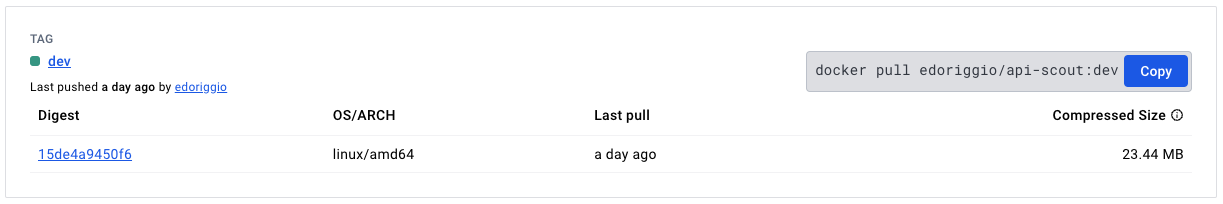
\includegraphics[width=0.9\linewidth]{assets/png/deployment/dev-deployment}
    \end{center}

    \caption{Example of a published Docker image}
    \label{fig:deployment-example}
\end{figure}